\documentclass{article}
\usepackage[francais]{babel}
\usepackage[UTF8]{inputenc}
\usepackage[T1]{fontenc}
\usepackage{graphicx}
\usepackage{fancyhdr}
\usepackage{eurosym}
\usepackage{color}
\usepackage{soul}

\pagestyle{fancyplain} \chead{}\lhead{\textit{Les Professionnels}} \rhead{\emph{\textit{Evasion}}}

\definecolor{pseudorouge}{RGB}{200, 50, 50}
\definecolor{pseudoblue}{RGB}{20,10,230}

\begin{document}
\thispagestyle{empty}
\begin{center}
 \fontsize{21}{21}{\textbf{Rapport de Soutenance 1 \vspace*{0.2cm}\newline\textit{Evasion}}}
\end{center}

\vspace*{0.7cm}

\begin{center}
 \fontsize{21}{21}{\textbf{- Les Professionels/}}
 \fontsize{21}{21}{\textbf{2013-2014 -}}
\end{center}

\vspace*{0.5cm}

\begin{center}

\includegraphics[scale=01.0]{evasion}
\end{center}

\vspace*{0.5cm}

\fontsize{14}{14}
\begin{center}
{Lenny \textcolor{pseudorouge}{\textit{"Le Noob"}} Danino - danino\_l}
\end{center}
\begin{center}
Louis \textcolor{pseudoblue}{\textit{"El Parain"}} Kédémos - kedemo\_l
\end{center}
\begin{center}
 Anatole \textcolor{pseudoblue}{\textit{"Totonut"}} Moreau - moreau\_a
\end{center}
\begin{center}
Khalis Chalabi - chalab\_k
\end{center}

\begin{center}

\includegraphics[scale=00.20]{infini}
\end{center}

\newpage
\thispagestyle{empty}
\tableofcontents

\newpage
\fontsize{12}{12}
\pagenumbering{arabic}
\section{Introduction}

\par
Cela fait un bon moment que nous attendions de pouvoir nous concentrer a fond sur notre projet et finalement nous y voila. Nous avions commence deja avant la fin de l'annee mais maintenant que les partiels et les controles sont passes l'occasion de prendre de l'avance pour le projet nous est possible. Cela permettra de revoir les erreurs ou modifications plus tot et d'ameliorer notre tres estime jeu.
\newline

\par
Comme nous l'avions dis dans notre cahier des charges, notre jeu consistera en un Beat'em Up dans lequel notre personnage principal, un prisonnier qui n'aurait jamais du l'etre,  s'echappe de sa prison et tente de rentrer chez lui par n'importe quel moyen et donc rencontre des gardes et des ennemis  qui le bloqueront dans son evasion. Ce jeu sera en vue 3D a la troisieme personne.
\newline

\par
Ainsi puisque notre gourmandise nous amena a une creation d'un autre niveau, il a fallu apprendre a utiliser des outils precis comme BLENDER mais surtout a bien manier le C\# et XNA ce qui ne fut pas tres facile pour tous mais les tutoriels ont ete tres pratiquent. Aujourd'hui encore des difficultes subsistent mais de bonnes ameliorations furent realisees.
\newline

\par
Par ailleurs, il a fallu nous organiser comme nous ne sommes pas dans les memes classes. C'est donc pour cela que nous utilisons GITHUB qui permet de voir l'ensemble de la progression du jeu mais aussi de recuperer le code et cela independemment de l'endroit ou l'on se trouve. Aussi nous avons monte un site internet sur notre jeu ou nous mettons l evolution de celui-ci, les progressions, les noms de ceux qui participent aux differentes parties et bien plus viendra par la suite.Nous restons constamment en contact, et nous partageons nos fichiers. Notre code est également organisé en sections et sous sections ce qui permet de coder de manière plus efficace tout en etant  plus lisible.
\newline

\par
Notre jeu n'est pas encore jouable mais le menu est visible et cliquable. Il est donc loin d'etre termine mais on peut deja avoir une vision de ce a quoi il ressemblera. Nos efforts finiront par etre recompenses mais pas encore!
\newline

\par
Parlons du groupe maintenant. Nous sommes une veritable equipe ou chacun peut compter sur les autres pour l'aider quelque soit le probleme. Malgre le fait que nos classes ne soient pas les memes nous faisons tout pour se voir un maximum et de partager nos idees sur le jeu ou meme sur tout et n'importe quoi !
\newline

\par
Voici donc le travail que nos avons effectue depuis nos debuts sur le projet et celui que nous executerons pour la prochaine soutenance.

\newpage


\subsection{Louis\textcolor{pseudoblue}{\textit{"El Parrain"}} Kedemos }

\subsubsection{Experience personnelle}

Depuis quelques mois maintenant, je travaille sur le projet avec Lenny, Khalis et Anatole. Et je dois bien avouer, c'est plus dur que ce que je ne pensais. Chacun a sa propre idée. Chacun a ses propres envies. Chacun veut faire ce qu'il lui plait. Mais ce n'est pas possible. Il m' fallut, comme les autres je suppose, faire de nombreuses concessions. Définir un projet qui plait à tout le monde est une chose ardue. De plus, trouver des horaires pour travailler ensemble sur le projet n'est pas facile non plus, chacun ayant ses obligations personnelles.

\subsubsection{Affichage et animation de la 3D}
La \bsc{3D} a représenté le plus dur jusqu'à maintenant. Au début, voyant l'abondance d'exemple sur internet, je me suis dis que faire de la 3D serait facile. Mais j'ai très vite déchanté. Plus je regardais ces exemples, plus je me voyais confronté à un mur. En effet, sur internet, il n'y a que des exemples pratiquement. Et aucune explication. Ou alors je ne sais pas chercher. Et dans ce cas là, la suite de l'année risque d'être bien compliqué. \\
La première étape dans l'affichage des éléments \bsc{3D} est bien évidemment d'avoir des éléments en \bsc{3D}. Ayant déjà manipulé \bsc{Blender}, je me suis mis à l'\oe uvre. Pour nos premiers test, un bonhomme cubique a été réalisé : \begin{center}
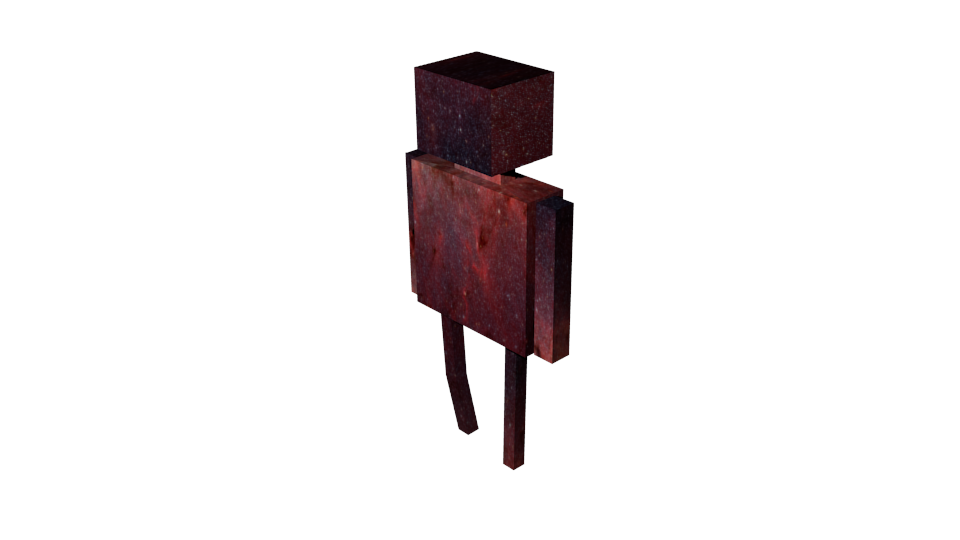
\includegraphics[scale=01.0]{perso}
\end{center}
Appliquer une texture, c'est à dire donner des couleurs à ce bonhomme, est très simple. L'image suivante montre le modèle \bsc{3D} avec chacune de ses faces aplatie : 
 \begin{center}
\includegraphics[scale=0.5]{UVmapping}
\end{center}
Il suffit de remplir chaque polygône avec la texture souhaitée pour habiller complètement le modèle.

Il est assez basique, mais malheureusement, je n'ai pas eu le temps de modéliser un vrai personnage. Cela demande du temps, une maîtrise plus poussée de \bsc{Blender}. N'ayant aucun des deux, j'ai préféré reporté cette tâche à plus tard pour me concentrer sur l'affichage et l'animation \bsc{3D}

Finalement, j'ai cherché des aides dans des vidéos, sur \bsc{Youtube} notamment. Une vidéo en particulier m'a permi de comprendre comment \bsc{XNA} permettait de gérer la \bsc{3D}. Une fois que l'on a compris qu'un modèle \bsc{3D} pouvait se charger en quelques lignes (sans compter l'affichage et ses transformations), la vie paraît plus simple : \begin{quote}
private Model persoModel;
\end{quote}

Manipuler un tel modèle implique de connaître les règles de base de la géométrie dans l'espace, mais aussi de savoir utiliser des matrices. En \bsc{3D}, tout n'est question que de matrices. \\
Par ailleur, lorsque le modèle est déplacé, la caméra devra sûrement le suivre dans son déplacement. Là encore il faudra faire intervenir des matrices de rotation et de translation.
\newline

Avec tout cela vient aussi une manipulation aisée du modèle. Il est possible de déplacer, tourner ou redimensionner le modèle \bsc{3D} comme on le ferait avec une image \bsc{2D}, via l'utilisation de \bsc{Vector3} : 
\begin{quote}
persoPosition = new Vector3(0f, 3f, 0f);\\
persoRotation = new Vector3(90.0f, 0f, 180f);
\end{quote}

Le plus gros problème que j'ai été amené à rencontrer en \bsc{3D} est l'animation d'un modèle. L'animation c'est le passage successif d'un état à un autre d'un modèle, par exemple un personnage qui marche, qui s'accroupi est une animation. Ce n'est pas un déplacement à proprement parler, car le modèle \bsc{3d} reste à la même place dans la fenêtre de jeu, mais son état change : 

 \begin{center}
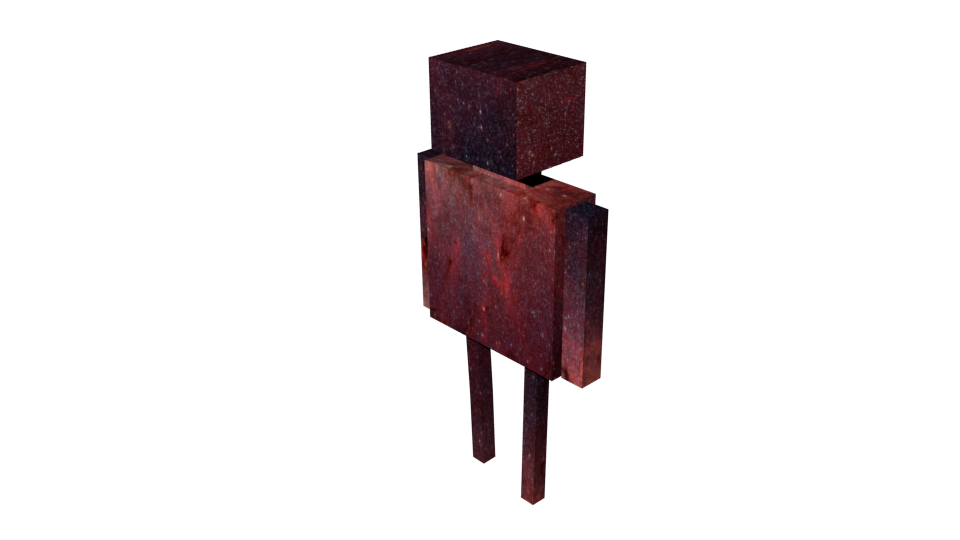
\includegraphics[scale=0.5]{static}
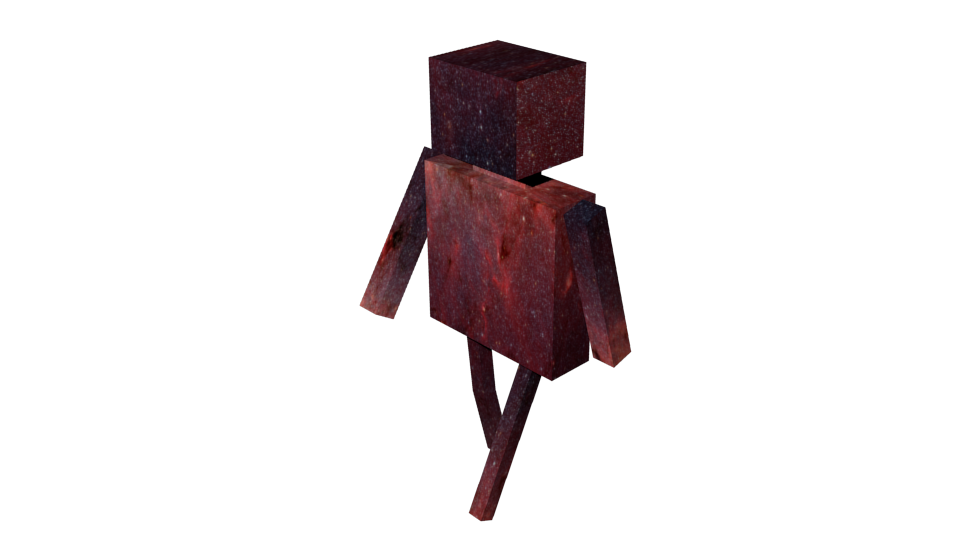
\includegraphics[scale=0.5]{MARCHE}
\end{center}

Effectuer ce genre de transformation est compliqué. Les matrices sont encore une fois utilisées. Un modèle \bsc{3D} est globalement composé de deux éléments : un squelette et une texture. La texture est ce qui recouvre le squelette, c'est ce que l'on perçoit du modèle. Le squelette permet de dire où placer cette texture pour donner l'impression d'un personnage en marche, ou encore d'un oiseau en vol. Sans squelette, notre modèle peut être affiché mais ne pourra pas etre animé.\\
Animé un modèle passe donc par l'animation d'un squelette. Et animer un squelette passe par l'utilisation de matrices. Ces dernières vont indiquer comment translater, tourner chaque os du squlette. On pourra ainsi animer chaque os, donc chaque partie du squelette, indépendamment des autres os. Tout comme notre squelette nous autorise à bouger chacun de nos membres.\\

\newpage
\begin{quote}
SkinningData skinningData = currentModel.Tag as SkinningData;

if (skinningData == null)\\
\hspace*{0.5cm}       throw new InvalidOperationException\\
\hspace*{1.0cm}             ("This model does not contain a SkinningData tag.");\\

\end{quote}

Ce bout de code peut sembler anodin, mais c'est celui ci qui pose le plus gros problème. Il m'a fait me rendre compte l'importance des \bsc{TAG} d'un modèle \bsc{3D}. Un \bsc{TAG} est une information de base sur le modèle \bsc{3D}. Cela concerne entre autre le nombre d'image de l'animation, le nombre d'animations du modèle, la hiérarchie du squelette... A ce stade du projet, l'animation n'a pas été intégrée, mais ce n'est pas pour autant qu'elle me résistera bien longtemps. La seule barrière entre le personnage statique et le personnage animé concerne le \bsc{SkinningData tag}. Sinon, je pense avoir tout les éléments en main pour bien comprendre et mettre en \oe uvre l'animation de modèles.  

\subsubsection{Le jeu en général}
Vous l'aurez compris, la partie \bsc{3D} représente la partie la plus importante de mon travail. Mais j'ai malgré tout réussi à participer aux autres éléments du jeu (sans trop avoir le choix).\\
Avec Anatole, nous avons construit une première ébauche assez satisfaisante du menu d'accueil : 

 \begin{center}
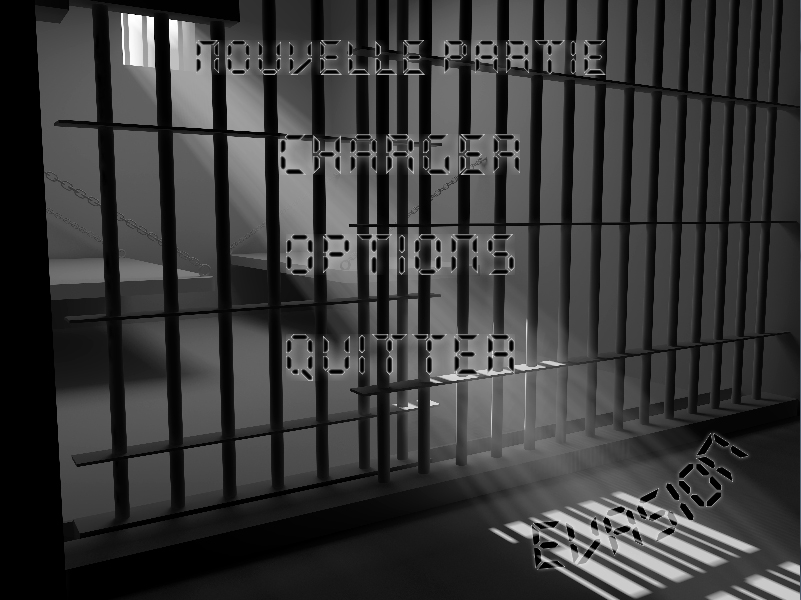
\includegraphics[scale=0.3]{menu}
\end{center}


Bien sûr, le menu sera amené à évolué dans le futur. Pour l'instant, seul le bouton "Nouvelle Partie" est actif. Les autres seront implémentés quand le jeu aura plus de contenu. Les boutons eux-mêmes seront améliorés, pour être moins statiques. Pour le moment, c'est une alternance entre deux images :

\begin{center}
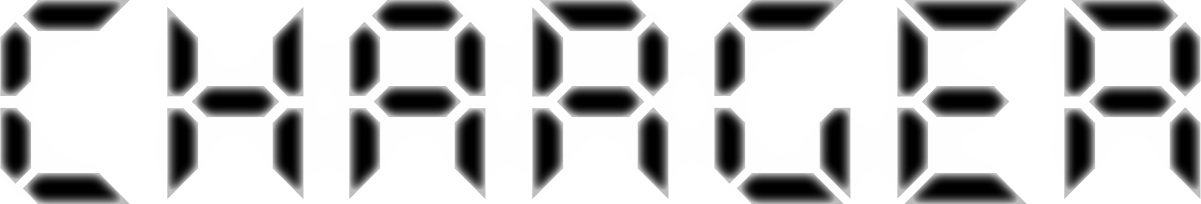
\includegraphics[scale=0.35]{off}
\hspace*{1.0cm}
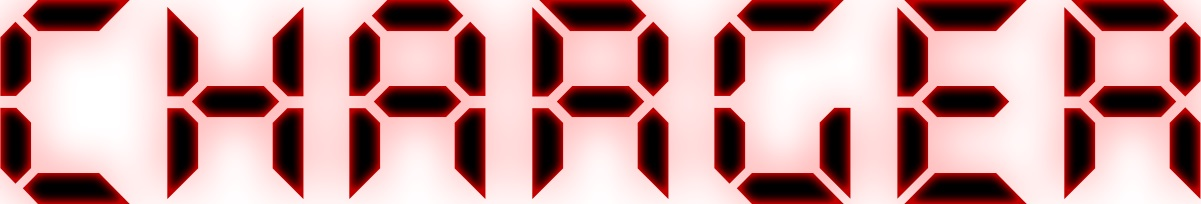
\includegraphics[scale=0.35]{on}
\end{center}

\newpage
J'ai aussi manqué de temps pour travailler l'identité visuelle du jeu. Peu de recherches graphiques ont été effectués. Nous avons décidé de construire un projet propre en premier lieu. Toute une arborescence de classes, de dossiers a été établie pour avoir un projet fort modulable. Ainsi chacun de nous peut travailler sur ce qui lui incombe sans se préoccuper de l'avancement des autres. Nous pourrons avancer à notre rythme. Ce point nous a semblé plus important que d'avoir des textures au début du projet. Commencer un projet bien organisé est mieux que de commencer un beau projet. De plus, si l'envie nous vient d'intégrer une nouvelle fonctionnalité au jeu, car il s'agit bien d'un jeu, ne l'oublions pas, la bonne organisation du projet va grandement faciliter cette intégration. C'est pour cette raison que pour la deuxième soutenance, une véritable charte graphique sera vous sera présenté.

\subsubsection{Et après ?}
\par
C'est la première fois que je réalise un projet de cette taille. Au début, j'ai sûrement vu trop grand. Je pensais avoir le temps de tout faire. Mais ça n'a pas été le cas. Il m'a fallu laisser de côté certaines parties du projet pour me concentrer sur d'autres, comme expliqué précédemment. C'est le cas des graphismes et de l'animation des modèles \bsc{3D}. 
\newline

\par
Maintenant, je que je sais à quoi m'attendre, je pense pouvoir mieux gérer mon temps et mon énergie pour la suite du projet. Il me reste beaucoup de travail. Il y a toute la partie graphique : les sprites \bsc{2D}, les modèles \bsc{3D}, les boutons des menus, un curseur adapté au jeu.


\par
Je devrais aussi implémenter un système de collision. Voir son personnage rentrer dans un mur peut en laisser plus d'un perplexe. Le personnage ne pourra évoluer que dans deux dimensions : aller en avant ou arrière, et sur la gauche ou la droite. On retire la dimension de la hauteur, donc tout ce qui est les sauts, les escaliers. J'utiliserai une méthode classique : la détection des collisions par rectangle. Si un rectangle entre en contact ou chevauche un autre rectangle, on estimera qu'il y a une collision. Voici un exemple : 

 \begin{center}
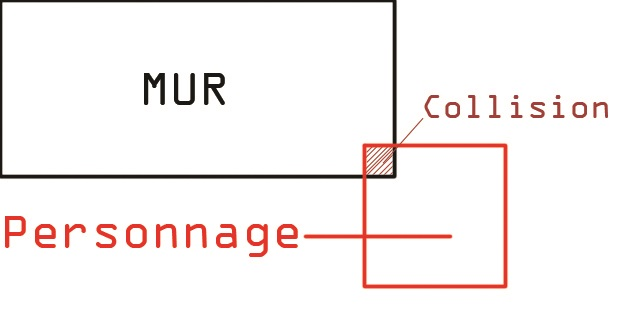
\includegraphics[scale=0.5]{collision}
\end{center}

Pour simplifier les tests, nous n'utiliserons que cette méthode. Pour faire les tests de collision, chaque élément du jeu sera ramené à une boîte rectangulaire. \\
\par
Enfin, nous devrons avoir bien commencé la boucle principale du jeu et l'intéraction entre les différents élements du jeu. C'est à ce moment que le jeu deviendra vraiment interactif. Les résultats se feront voir petit à petit. 
\\
La partie réseau, si nous travaillons bien jusque là, devra être terminée. A première vue, elle ne présente pas de grande difficultés. Une simple communication avec un serveur est à prévoir. Donc pas de dialogue entre deux ordinateurs (OUF !).
\newpage

\subsection{Khalis Chalabi}

\subsubsection{Avancement du projet}

Dans cette partie je vais vous présenter dans un premier temps les recherches que j’ai dû effectuer pour pouvoir m’occuper des parties qui m’étaient destinées puis les différentes tâches que j’ai  accompli pour cette première soutenance, et enfin les problèmes que j’ai rencontré.
\newline

\par
\underline{Acquisition de connaissances en programmation web et en C\# :}
\newline

\par
Comme vous aviez pu le lire dans ma présentation figurant dans notre cahier des charges, l’informatique et moi c’est une histoire qui commence tout juste ! Donc en tant que débutant je n’avais pas l'intégralité des connaissances requises pour pouvoir exécuter pleinement les tâches que mon groupe m’avait confiées. Il est vrai que les TPs effectués depuis le début de l’année me fournissaient quelques bases mais ce n’était pas suffisant pour ce que je devais et ce que je voulais faire. Pour cette première soutenance je devais implémenter plusieurs classes, faire bouger un personnage 3D et je m’étais fixé comme objectif acquérir des bases en développement web pour pouvoir commencer à développer un site.
\newline

\par
Les TPs réalisés au cours de l’année m’ont permis d’implémenter les classes Personnages, Objets et Décors. Cependant, faire déplacer un personnage 3D à l’aide du clavier me dépassé complètement. Je me suis donc mis à la recherche d’un tutoriel qui allait pouvoir me permettre d’effectuer ma mission ! Le site du Zéro étant le plus grand ami des débutants, je me suis directement rendu sur ce site. Et j’ai bien sur trouvé un tutoriel qui me convenait parfaitement : ''Le développement de jeu vidéo avec XNA'' ! A première vu ce tutoriel semblait parfait pour moi vu que notre jeu vidéo devait fonctionner sous XNA. En effet, il était parfait. Ce tutoriel était plutôt simple et assez court si on avait déjà quelques bases en  C\# ce qui était mon cas. Il rappelait pour commencer ce qu'était XNA et ce qu'on pouvait faire avec ce framework. Puis il expliquait l'utilisation des sprites et pour finir comment faire interagir une image avec le joueur. Vous l'avez sûrement compris, il est ici question de 2D. Cependant, ce tutoriel m'a grandement aidé pour comprendre comment faire bouger une image avec les touches du clavier ou une souris. J'avais donc enrichi mes connaissances en programmation et pouvais commencer à essayer de faire bouger mon personnage 3D.
\newline

\par
Lors de la 2ème soutenance il est obligatoire de présenter un site web. Un membre de notre groupe : Anatole dit Totonut possédais déjà les connaissances nécessaires pour la création d'un site web. Cette partie m'intéressais je lui ai donc proposé de nous occuper du site web ensemble.  Cependant, encore une fois je ne connaissais strictement rien sur la création de site web si ce n'est que cela demandais l'utilisation de HTML et CSS, deux langages web. Chouette encore de nouveaux langages à apprendre ! Le site du Zéro me fût encore d'une très grande aide car c'est grâce à celui-ci que je pu apprendre les bases de HTML5 et de CSS3. J'étais particulièrement content car une fois qu'on a fait du Caml et du C\# le HTML et le CSS c'est plutôt de la rigolade !
\newline

\par
\underline{Implémentation des classes Personnages, Objets et Décors :}
\newline

\par
Un jeu vidéo sans personnage, sans objets (armes, trousse de secours, lampes torches...) et sans décors c'est moche... Et c'est à ce moment-là que j'entre en jeux ! Comme je vous l'ai précisé dans les paragraphes précédents, mais sans entrer dans les détails, j'étais chargé d'implémenter les classes Personnages, Objets et Décors. Parmi les tâches qui m'étaient attribuées j'ai décidé de commencer par celle-ci car grâce aux TPs, je savais ce qu'était une classe et comment cela fonctionnait. Cependant il n'y avait pas juste trois classes à implémenter mais beaucoup plus ! En effet la classe Personnage était la classe mère et elle possédait des classes filles : la classe Ennemi, la classe Joueur ainsi que la classe PNJ (personnages non jouables). Et il en était de même pour les classe Objets et Décors elles possédaient chacune plusieurs classes filles.
\newline

\par
La classe, mère, Personnages et ses classes filles furent les  plus longues et les plus dures à coder. Elles comportaient plusieurs fonctions et les constructeurs étaient assez longs. Après avoir bien compris la logique les classes Objets et Décors ainsi que leurs classes filles  ne furent pas très difficile à implémenter. J'ai pu tester mes connaissances grâce à ce travail et cela m'a permis de revoir ce que j'avais déjà fait en TP (constructeurs, héritage, énumérations ...)   
\newline

\underline{Déplacement du personnage 3D :}
\newline
\par
Le déplacement du personnage 3D fût la tâche la plus difficile à exécuter vu qu'il fallait interagir avec le joueur et que ce n'était pas une notion que nous avions abordé en TP. Comme je vous l'ai dit précédemment j'ai suivi un tutoriel sur le site du Zéro. Le tutoriel était destiné à un jeu en 2D mais cela ne changeait pas grand-chose au déplacement du personnage en 3D. J'ai pu apprendre en plus l'utilisation des sprites qui ne me serviront pas ici cependant. En 3D nous utilisons un modèle. Je pensais que cette partie allait être assez difficile mais finalement ce n'était pas très compliqué. Il me suffisait juste de récupérer l'était du clavier et en fonction des touches qui étaient enfoncés faire varier la position du personnage 3D ainsi que sa vitesse.  Cette tâche, contrairement à ce que je pensais ne fût pas la plus difficile à effectuer.
 Il ne faut cependant pas penser que mon travail fût sans difficultés, j'ai rencontré quelques problèmes...    
\newline

\par
\underline{Problèmes rencontrés :}
\newline
\par
Ce projet est mon premier gros projet en groupe en informatique. Je savais d'avance que ça n'allait pas être facile et j'ai en effet rencontré plusieurs problèmes plus ou moins importants. Heureusement pour nous nous sommes un groupe assez organisé, nous avions donc sur papier la majorité de nos idées : de quelles classes nous allions avoir besoin, avec quels attributs et quelles méthodes. Cependant malgré cela j'ai dû faire face à un problème majeur : le problème du ''il y a toujours quelque chose à rajouter ou à modifier'' ! Ce fût pour moi une des choses les plus difficile à gérer, il y avait toujours une méthode, un attribut, une classe ou un constructeur à rajouter ou à modifier dans notre code. A chaque fois que je pensais avoir fini je me rendais compte que finalement il manquait un petit quelque chose. Et je peux vous dire que ça a de quoi fatiguer !
\newline

\par
Le manque de connaissances est également une difficulté à laquelle, nous, les débutants sommes confrontés. Il faut sans cesse se documenter, faire des recherches, suivre des tutoriels pour pouvoir avancer dans le projet. Mais je pense que c'est un mal pour un bien, en effet cela nous prend du temps et ce n'est pas toujours facile avec l'école et les devoirs, mais nous progressons d'avantage. De plus nous obtenons une réelle satisfaction à réussir quelque chose dont nous étions incapables  quelques semaines avant cela.
\newline

\par
J'aurais bien voulu aider un peu plus pour la 3D mais c'est assez compliqué et j'ai vraiment du mal à comprendre. J'essayerai d'apporter un peu plus d'aide pour la 3D pour la prochaine soutenance mais ce n'est pas quelque chose de facile pour un débutant je ne garantis donc rien.
\newline

\subsubsection{Et après ?}
\par
Pour cette deuxième soutenance je vais me fixer plusieurs objectifs à atteindre :
\newline

\par
\underline{Amélioration du site et Finalisation des classes:}
\newline
\par
Nous sommes un peu en avance sur cette partie vu que le site web n'est censé être présent qu'à partir de la deuxième soutenance. Ceci dit il n'est pas parfait et je vais tenter de l'améliorer avec l'aide d'Anatole.
Aussi je m'occuperai de finir complètement les classes Personnages, Objets et Décors car elles ne sont pas finies. Il reste une ou deux classes filles à implémenter pour chacune des classes mères.
\newline

\par
\underline{Début du mode multijoueur :}
\newline
\par
Je pars encore une fois à l'aventure car je ne sais pas du tout comment m'y prendre pour créer un mode multijoueur. Un travail de recherche va donc devoir être effectué pour cette partie.
\newline

\par
\underline{Premiers pas en 3D :}
\par
Je vais essayer d'apporter mon aide pour la 3D, je pense que cet objectif sera le plus dur à atteindre.

\newpage

\subsection{Lenny \textcolor{red}{"Le Noob"} Danino}
\subsubsection{Personnages/Decors}

\par
\underline{Les attributs des personnages}
\newline

\par

\underline{Les differents decors}
\newline

\newpage

\section{Modification du planning}

Avec les légers changement de direction que nous avons pris, le planning initialement établi a dû être quelque peu modifié pour coller au plus près de l'avancement de notre projet. C'est ainsi que les graphismes ne commenceront à être développé que pour la deuxième soutenance. En revanche, certains domaines ont été plus facile à réaliser. Nous avons pu prendre une certaine avance notamment dans la réalisation du site web et des sons. A l'avenir, nous pourrons nous concentrer avec plus d'ardeur sur les points importants.
\begin{center}
\begin{tabular}{|c|p{2cm}|p{2cm}|p{2cm}|}


\hline
   & Première soutenance & Deuxième soutenance & Troisième soutenance\\ 
\hline

Codage décors & 70\% & 100\% & 100\%\\
\hline
Codage objets & 70\% & 100\% & 100\%\\
\hline
Codage personnages & 70\% & 90\% & 100\%\\
\hline

Graphismes 2D/3D & - & 60\% & 100\%\\
\hline

Site web & 70\% & 100\% & 100\%\\
\hline

Son & 20\% & 80\% & 100\%\\
\hline

Collisions & - & 50\% & 100\%\\
\hline

Affichage & 70\% & 100\% & 100\%\\
\hline

Boucle de jeu & - & 50\% & 100\%\\
\hline

Interaction entre éléments du jeu & 20\% & 70\% & 100\%\\
\hline

Menu & 50\% & 100\% & 100\%\\
\hline

Réseau & - & 100\% & 100\%\\
\hline

Multijoueur & - & 60\% & 100\%\\
\hline

\end{tabular}
\end{center}

\section{Conclusion}

\par
C'est donc apres beaucoup de travail  pendant ces 3 mois que nous continuons notre projet en espérant que nous tiendrons nos objectifs. Nous restons tres motivés pour le terminer, et pensons constamment à de nouvelles améliorations et des perfectionnements. Notre travaille reste dur et le devient de plus en plus en fonction de notre avancement.
\newline

\par
Maintenant place à la présentation de notre projet durant la première soutenance !

\end{document}